\section{Implementation}

In this section, we discuss the implementation of all languages and transformations related to \SLCO.
The tools used to implement these languages and transformations are described in more detail in Appendix~\ref{ap:tools}.
All the grammars, metamodels, and transformations described below are available online\footnote{\url{http://code.google.com/p/simple-language-of-communicating-objects/}}.

Figure~\ref{fig:slco:implementation-overview} gives an overview of the languages and transformations related to \SLCO.
In this figure, all languages that are based on a metamodel implemented using the Eclipse Modeling Framework (EMF)~\cite{Steinberg2008} are depicted as rectangles.
The rounded rectangles represent languages that have a textual concrete syntax, and the arrows represent model transformations, parsers, and template-based code generators, which either transform models or convert them from one representation to another.

\begin{figure}[hbt]
\centering
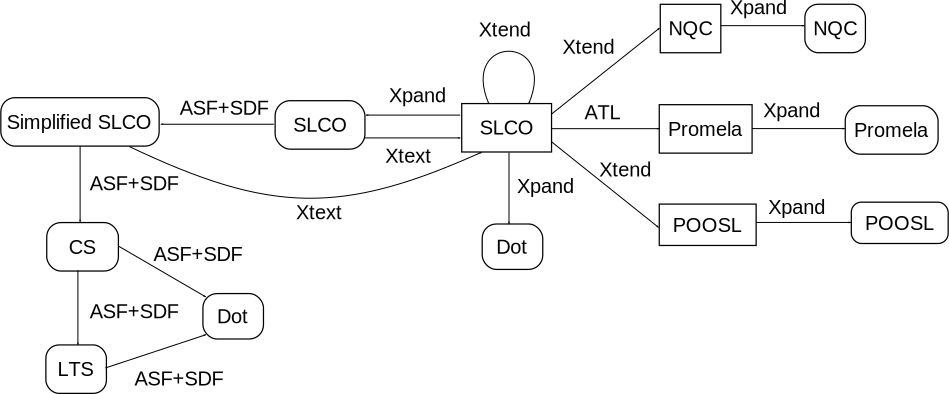
\includegraphics[scale=.49]{iterative-dsl-evolution/figs/overview}
\caption{Overview of languages and transformations}
\label{fig:slco:implementation-overview}
\end{figure}

The metamodels of \SLCO, \NQC, \Promela, and \POOSL define the abstract syntax of these languages.
They define the concepts offered by the languages and the relations between these concepts.
To enable creation of models, EMF offers the automatic generation of a tree-view editor from metamodels.

Unfortunately, creating large models using the standard editor provided by EMF is cumbersome.
To ease the process of modeling, we defined a textual syntax for \SLCO with \Xtext~\cite{Efftinge2006xText}, which also provides us with a textual editor for \SLCO.
Since all other models are automatically generated from \SLCO models, there is no need for convenient editors for the other languages involved.

All endogenous transformations that are used to bridge the gaps between \SLCO, \NQC, \Promela, and \POOSL are implemented using the \Xtend model transformation formalism~\cite{Haase2007OAW}.
In Figure~\ref{fig:slco:implementation-overview}, these transformations are represented by the arrow that connects the rectangle labeled \SLCO to itself.
The transformations from \SLCO to \POOSL and \NQC are also implemented using \Xtend, and the transformation from \SLCO to \Promela is implemented using the ATL Transformation Language~\cite{Jouault2005}.

The result of each of these transformations is a model that conforms to the corresponding metamodel.
These models cannot be used directly in \POOSL and \Spin or on the Lego Mindstorms platform.
Instead, models in textual form are required for simulation, verification, and execution.
Therefore, we implemented model-to-text transformations for these tools using \Xpand~\cite{Haase2007OAW}.
Additionally, \Xpand is used to produce the diagrams that form the graphical syntax of \SLCO.
Each of the diagrams is in fact a directed graph written in \DOT that can be visualized with the \graphviz tool~\cite{Ellson01graphviz}.

The textual languages \CS and \LTS, their relation to \DOT, and the transformations implemented in \ASFSDF~\cite{Brand:2001:ASF} are discussed in detail in Chapter~\ref{chap:prototype-semantics}.
The relation between these languages and the simplified version of \SLCO discussed in Section~\ref{sec:SLCO:simplified_slco} is also described in Chapter~\ref{chap:prototype-semantics}.
Because every textual model that is expressible in the simplified version of \SLCO is also expressible in the regular version of the language, the parser and editor that are generated from the \Xtext grammar of \SLCO are also suited for the manipulation of simplified textual \SLCO models.
